\documentclass[ukenglish]{nik}  

%NIK packages
\usepackage{times}

\usepackage[latin1]{inputenc}
%angir tegnsettet i LaTeX-filen. (Opsjonen m� selvf�lgelig tilpasses om man har et annet tegnsett.)
\usepackage[T1]{fontenc}
%spesifiserer bruk av 8-bits fonter.
%\usepackage{babel}  comment SH (only needed for Norwegian I suppose)
%ordner alle spr�kavhengig ting.
\usepackage{textcomp}
%gir tilgang til flere symboler.
\usepackage{type1cm}
%forteller at systemet kan skalere Computer Modern i alle st�rrelser. 	

%spesific packages
\usepackage{graphicx}				
\usepackage{array}								
\usepackage{amssymb}
\usepackage{cite}
\usepackage[final]{fixme}
\usepackage{pdfpages}
\usepackage{tabularx}


\title{Requirement Engineering for a Small Project with Pre-Specified Scope}
\author{Thomas D.\ Nielsen, Sigve Hovda, Andr\'es Masegosa, Helge Langseth, \\
Antonio Fern\'andez, Antonio Salmer\'on, and Anders L.\ Madsen} 
\date{Latest version, \today}		%To be excluded later					
\begin{document}

\maketitle

\begin{abstract}
There is a general lack of formal and agreed upon methods for conducting requirement engineering (RE) for smaller software projects \cite{Ara07,Qui10}.  Many small projects have a pre-specified scope, since the pre-specified scope often appears when the project needs to agree with a grant agreement that partially funds the project.  To our knowledge, there exist no publications on small projects where the scope is specified before the project is started.  

In this paper, the RE process is outlined for the project named: Analysis of MassIve DataSTreams (AMIDST).  AMIDST is a project that is partially funded by the European Union's Seventh Framework Programme for research, technological development and demonstration.  This project has a pre-specified scope, because the grant agreement demands that a requirement engineering process is conducted within a specified time frame and also that the result of the requirement process is in compliance with the Description of Work (DoW) that is agreed upon.   

The AMIDST RE process is based on selected methodological approaches from existing RE processes, which subsequently have been tailored to the specific characteristics of the AMIDST project.  The characteristics in the AMIDST project are; there exist a pre-specified scope, partners are located far apart, massive knowledge transfer between parners is expected, the software framework need to be applicable in three different industrial domains and that it is expected that the project focus will be refined.  

In general, a use-case driven approach is followed, because functional requirements are in focus. Another important tool in the AMIDST RE process is the development of a unified and formal template for elicitation to encourage the overall transparency of the process.
\end{abstract}

\section{Introduction}

The requirements engineering (RE) process adopted by a particular software project typically reflects intrinsic
characteristics of the project in question. Thus, there is often no standard way to conduct a RE process \cite{Poh10},
but one rather adapts existing processes to the needs and specifics of the project. This especially applies to smaller
software projects \cite{Qui10,Ara07}, where the RE processes follow
more ad-hoc strategies and a best practice seems to be lacking. 

In this paper, the RE process for the project entitled \emph{Analysis of MassIve Data STreams} (AMIDST) is outlined. AMIDST is a
project that is partially funded by the European Union's Seventh Framework Programme for research, technological
development and demonstration, and falls in the category of a small development project. AMIDST has a pre-specified
scope, because the grant agreement asserts that the result of the RE process must be in compliance with the \emph{Description
  of Work} (DoW). The DoW defines the scope of the project as well as more general requirements to the system, both
functional and non-functional, and e.g.\ includes a fixed deadline for the RE process. The latter restricts the project from,
e.g., following a strict agile approach \cite{Din10},  where a product owner is continuously renegotiating the
requirements and where the RE process is seen as a continuous process throughout the whole project
\cite{Kav11}. Furthermore, the software framework developed in the project should be sufficiently general to accommodate
stakeholders and use case providers representing different industries. Thus, the RE process relates not only to the software framework, but also to the solutions to be developed
for the use cases of the project. Specifically, for each use case provider the general AMIDST framework will be instantiated in order
to meet the needs and requirements of that use case provider. 

To the best of our knowledge, there exist no guidelines for the RE process for small projects with these
characteristics. This paper therefore  attempts to make a first step towards defining a best practice for such
situations. The project's characteristics and challenges have formed the basis for the development of the AMIDST RE
process. Based primarily on organizational characteristics of the project, the RE process is composed of selected
components from existing RE processes that have been tailored to the identified AMIDST characteristics. However, we
believe that the characteristics are sufficiently general to make them applicable for other small projects. In particular, it is expected that projects that share at least some of the characteristics of the AMIDST project may draw on the methodology that is outlined in this paper.

The paper is outlined as follows. In section  \ref{sec:stateOfArt}, the basic principles of requirement engineering are briefly outlined. Section  \ref{sec:AmidstRequirementProcess} starts by describing the main characteristics of the AMIDST project, before the RE process is presented. In section  \ref{sec:realization}, we have described the realization of the process, and the report is concluded in section  \ref{sec:conclusion}.


\section{Basic principles in requirement engineering}
\label{sec:stateOfArt}

In practice, the requirement engineering process ends with a document containing a list with requirements, which are in the form of what a software must do or comply with.  

To date there is no common definition of requirement engineering.  Some definitions focus on elicitation of requirements and therefore the interaction with the user, while others focus on the documentation or the specification.  A definition that takes both focuses into account is the IEEE standard given in \cite{Iee90}:

\emph{
\begin{enumerate}
\item The process of studying user needs to arrive at a definition of system, hardware or software requirements.
\item The process of studying and refining system, hardware or software requirements.
\end{enumerate}
}

In the context of understanding the requirement engineering process, it is worth spending some space on defining the requirement itself.  A definition of a requirement is given in IEEE standard \cite{Iee90}: 
\emph{
\begin{enumerate}
\item A condition or capability needed by a user to solve a problem or achieve an objective. 
\item A condition or capability that must be met or possessed by a system or system component to satisfy a contract, standard, specification or other formally imposed document. 
\item A documented representation of a condition or capability as in 1 or 2.
\end{enumerate}
}

This definition has a clear focus on the user, the system/system component and also which contract, standard or specification is needed to be met. Notice, that the requirement is related to \emph{what} a system can do and not \emph{how} it is done.

\subsection{Activities involved in requirement engineering}

The activities involved in requirements engineering vary widely, depending on the type of system being developed and the specific practices of the organization(s) involved  \cite{Som11}.  These may include:
\begin{itemize}
\item Requirements inception or requirements elicitation 
\item Requirements identification - identifying new requirements
\item Requirements analysis and negotiation - checking requirements and resolving stakeholder conflicts
\item Requirements specification (Software Requirements Specification) - documenting the requirements in a requirements document
\item System modeling - deriving models of the system, often using a notation such as the Unified Modeling Language
\item Requirements validation - checking that the documented requirements and models are consistent and meet stakeholder needs
\item Requirements management - managing changes to the requirements as the system is developed and put into use
\end{itemize}

These activities are sometimes presented as chronological stages although, in practice, there is considerable interleaving between them.  

\subsection{Use case driven requirement engineering}

It has always been a challenge for the software industry to communicate functionality to the users of a software. Moreover, software engineers are often frustrated, because users often do not know what they want. They only have an idea of what they want.  To improve this communication, the use-case driven approach was developed in the nineties.  It was first published by Ivar Jacobsen \cite{Jac92} and more modern references are \cite{Poh10} and \cite{Coc01}.  A use case focuses only on the interaction between a user and the system.  Requirements are always associated with a use case. This means that the user is requested to only focus on what he/she wants.  This is an advantage, compared to the traditional way where requirements are listed in relation to components and subcomponents in the software.  The traditional way often lead to a complexity that the user do not understand.  Also, it is more common with requirement duplicates in the traditional approach.

A use case is a list of steps, typically defining interactions between an actor and a system, to achieve a goal. The actor can be a human or an external system.  An overview on how to write effective use cases is given in \cite{Coc01}, where several templates are given. The use case providers are asked to provide the use cases in natural language and for each use case the following questions are central:

\begin{enumerate}
\item Who are the actors involved in the use case? An actor is either a person or an entity that interacts with the software.  
\item What is the main event that initiates the use case? This could e.g. be an external business event or a system event that causes the use case to begin.  It could also be the initial step in a normal work flow. 
\item What are the main user actions and system responses that will take place during the normal execution of the use case?. This dialog sequence will ultimately lead to accomplishing the goal that is implied by the use case name and description.
\item How can we evaluate the success of the use case?
\end{enumerate}
 
It is also common to group the users, or human actors, within an organization into a small set of user groups. The users within each user group need to have similar roles within their organization and their set of competences are expected to be similar. 

To understand the use case driven approach to requirement engineering better, it is useful to distinguish between functional and non functional requirements.  Functional requirements are those requirements that are directly related to the interaction between the user and the system.  The non functional requirements are more hidden for the user are related to the global overall success.  For instance scalability, traceability and testability.  When use cases are provided and functional requirements are identified, it is the requirement engineers role to identify, document and communicate these non functional requirements as well.  The use case driven approach to requirement engineering focuses on revealing the functional requirements together with the users.  This improves the communication between the users and the developers, because the focus is on what the users wants and less on how it can be done.


\section{The AMIDST requirements engineering process}
\label{sec:AmidstRequirementProcess}

This section contains a description of the AMIDST RE process.  We first give a brief overview of AMIDST and describe the 
main characteristics of the AMIDST project that has influenced and shaped the RE process. Based on these characteristics 
we present the AMIDST RE process, which is based on the RE processes described in Section~\ref{sec:use-case-driven}, 
but tailored to the specific characteristics of AMIDST. Since the focus of the present RE process is on the functionality and 
documentation of the software products being developed, we will, e.g., not cover process-related requirements or non-
functional requirements, c.f.\ Section~\ref{sec:use-case-driven}. Non-functional requirements are defined by the
aforementioned DoW. 

\subsection{The AMIDST project: a brief overview}

AMIDST is a project funded by the European Union's Seventh Framework Programme for research technological development
and demonstration. The objective of AMIDST is to develop a scalable toolbox capable of providing a framework that
facilitates efficient prediction and data analysis in streaming data. The toolbox will be instantiated to target three
distinct industries represented by the three industrial use case providers in the AMIDST consortium. The use case
provider in the energy domain is Verdande Technology, the use case provider in the financial domain is the Cajamar Cajas
Rurales Unidas, and the use case provider in the automobile domain is Daimler AG.  In addition to the use case
providers, there are also three academic partners and a fourth industrial partner in the software industry.  The fourth
industrial partner is Hugin Expert and the three academic partners are the Norwegian University of Science and Technologogy, Universidad de Almeria, and Aalborg University.

The development of the toolbox and its subsequent instantiation will be driven by functional requirements specified by the use case providers and elicited in accordance with the RE process described in the present document; the requirements supplement the non-functional requirements described in the DoW framework. If deemed effective, the instantiated toolboxes (referred to as AMIDST \emph{solutions}) will be adopted by the use case providers. 

The AMIDST project is structured around ten work packages. The first work package is concerned with requirements
engineering and evaluation. Work packages 2--4 focus on methodological developments to be applied on the massive data streams.  In particular, there is emphasis on probabilistic models as well as scalable inference and learning
algorithms tailored to these models. Work package 5 is concerned with extensions to the AMIDST solutions to the Hugin software toolbox, which is already commercially available.  In Work packages 6--8 the AMIDST solutions for the three industrial partners will be realised. Finally, Work packages 9 and 10 deal with dissemination and exploitation as well as management.     

\subsection{Characteristics of the AMIDST project}
\label{sec:characteristics}

In this section we identify and describe the key characteristics of the AMIDST project that directly influence the 
requirements
engineering process. 

\ \\
\noindent \emph{Characteristics one:  Pre-specified scope of the project}
\label{sec:characteristic1}

The AMIDST project is funded by the European Union's Seventh Framework Programme for research, technological
development, and demonstration. The overall scope and main developments in the project are therefore defined from the
beginning of the project period and documented in the Description of Work. This will henceforth be referred to
as the DoW framework. More detailed requirements pertaining
to the functionality and documentation of the developed software should thus fit within the DoW framework, and their
necessity in relation to AMIDST should be justified and demonstrated.   


 

\ \\
\noindent \emph{Characteristics two: Partners at different geographical locations}
\label{sec:characteristic2}

The AMIDST consortium consists of 7 partners/stakeholders, 4 industrial and 3 universities, which are situated in 4 different
countries. This diverse consortium composition has at least a two-fold impact on the RE process.

First of
all, although AMIDST targets the industrial stakeholders' common need for processing massive data streams, the more
intrinsic aspects of the three industrial domains differ significantly. This, in turn, means that the partners will have different
(possibly conflicting) requirements for the system being developed. To ensure that the requirements are comparable
across domains and abide to the DoW, a unified formal framework for eliciting system requirements is needed. Such a
framework may also provide transparency in the overall requirement engineering process and help prioritize requirements
across different domains and thereby help resolve potential conflicts.   

Secondly, with the project partners located in different countries, there is a need for a controlled and stringent requirements
process in order to limit travel expenditures. This approach is supported by a unified formal requirements
engineering framework. Consultancy and discussions in relation to the
requirements will primarily be achieved through telecommunication conferences and by physical meetings only secondarily. 
% 
%% The result is a project with many stakeholders, which have different backgrounds, priorities and influences on the 
%software. Moreover, the partners are located in different countries, which implies that the financial and time costs for 
%personal meetings are quite high.  This characteristic has an influence on the pursued RE process, because the process is 
%restricted to not rely heavily on meetings with many participants.

\ \\
\noindent \emph{Characteristics three: Transfer of domain knowledge between partners}
\label{sec:characteristic3}

The industrial partners of the AMIDST project come from very different domains: the automotive, energy, and finance
industry. To ensure the development, refinement, and completion of the unified formal requirements framework it is
necessary with regular and structured communications among the project partners during the RE
process. This not only relates to the specific requirements, but also to the software and user context in which the
AMIDST framework should be deployed. The latter part, in particular, is required for a proper evaluation and validation
of the elicited requirements.


% On one side, it was essential that the industrial partners gained enough insight of what can be done with
% probabilistic graphical models to identify proper use cases.  On the other side, it was essential that the academic
% partners gained enough knowledge about the industrial domains to understand the proposed use cases and 
%requirements. 
%This was considered in the way we divided our work among the academic partners. 

\ \\
\noindent \emph{Characteristics four:  One framework for three different domains}
\label{sec:characteristic4}

The AMIDST toolbox should define a general framework that can encompass the diverse domains of the three industrial
partners. Thus, the format of the unified requirements framework should be sufficiently general and flexible to
allow for all relevant requirements to be elicited for the three domains. At the same time the framework should be
appropriately structured and formalized enabling a controlled elicitation process (see also Characteristic two) with the
requirements specified in a consistent manner making them comparable across domains. In order to also provide a basis 
for a controlled and
balanced system development, the requirements should be linked to
relevant project phases, work packages, and tasks. This, in particular, will provide the work package leaders with
a clear overview of the requirements that are relevant for the activities in a specific work package.   
%
%%One single framework shall solve all posed problems.  It is therefore a challenge to find common requirements that are 
%addressing problems across all three domains.
%

\ \\
\noindent \emph{Characteristics five: Potential refinement of project focus}
\label{sec:characteristic5}

AMIDST is an RTD project, where both the industrial and academic partners' understanding of the domains develop as
the project unfolds. In order to support a potential refinement of the project's focus and goals, the requirements
engineering process should allow for an internal (re)prioritization of the requirements that is transparent across
application domains.    


% The posed problems are challenging and, as usual, some aspects of the problems are not fully understood at this stage 
%in the project. We realize that the priority of some of the requirements can change as the project continue. There is also an 
%uncertainty related to how satisfied the industrial partners will be when the proposed solutions are implemented.  

%Defining a requirement is linked with the perception of which design pattern to follow \cite{Ral13}.  A design pattern is 
%chosen by the software %developer and is basically the path to meet the requirement.  As explained in \cite{Ral13}, when 
%there is a high degree of unclarity of which  design %pattern to follow, this ambiguity is transferred to the definition of the 
%requirement as well.  The goal of the AMIDST software is to reach targets %that are highly innovational, meaning that it is 
%particularly difficult to define requirements that are clear and unambiguous.
%

\subsection{Project phases and AMIDST requirements identification }

%% We decompose the overall project period into phases to better -> support identification of requirements and work
%% package allocation.

The overall project duration will be decomposed into different phases, each having distinct requirements. According to
\cite{Eig09} a project's life cycle can be divided into three general phases: the design phase, operations phase, and
disposal phase. The disposal phase is outside the scope of AMIDST and, thus, will not be considered in the present
document. The design and operations phase, however, represent the
temporal development of the project, and are initiated by the start of the project and ends with the testing of the
deployed system, which will be adopted by the use case providers if deemed effective. Each
phase can furthermore be described as a collection of distinct stages in the project. The overall process is
illustrated in Figure~\ref{REprocess2}. 

%
%%%In order for a requirement to be useful for the software engineers, they are often associated with steps in a product life 
%cycle as for instance described in \cite{Eig09}.  In this reference the overall life cycle is divided into three phases; design 
%phase, operation phase and disposal phase.  In the AMIDST software, the disposal phase is not relevant for us.  

\begin{figure}[htbp]
\centering
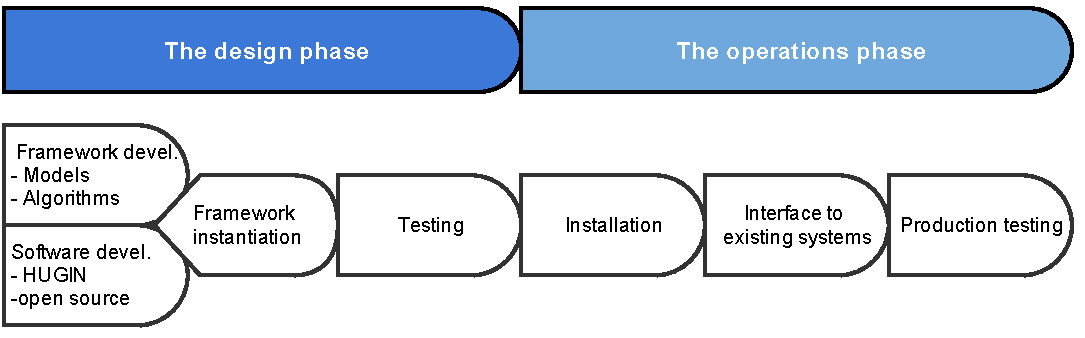
\includegraphics [keepaspectratio,width = 14cm] {amidst_phases}
\caption{The figure shows the key stages in the design and operations phases. For the requirement specification, each
  requirement should be defined relative to one of these stages.} 
\label{REprocess2}
\end{figure}


%\fixme{Describe the content of the two phases, design and operations}


In the design phase  general functionality requirements for the system are specified, i.e., what the system should do and 
support.
Figure \ref{REprocess2} details key stages inside this phase. The first stage consists of the design of the general
framework (models and algorithms) as well as the design and development of the software tools. These stages are 
primarily
related to Work packages 1--5. In the second stage, the general framework and software is instantiated for each specific
use case. Finally, initial tests of the use case instantiated frameworks are conducted.  During this phase of the project, 
possible design requirements could, e.g., address
\begin{itemize}[itemsep=2pt,parsep=2pt,topsep=4pt, partopsep=4pt]
 \item the scope of the model
 \item the interpretability of the learned models
 \item the extent and type of domain knowledge that can be integrated into the models
 \item prediction accuracy of the developed models
 \item documentation
\end{itemize}

The requirements for the operations phase concern the functionality of the deployed system. In Figure \ref{REprocess2}, 
we decompose this phase into three stages: installation, interface to existing systems, and production testing. The 
requirements for this phase could, e.g., address
\begin{itemize}[itemsep=2pt,parsep=2pt,topsep=4pt, partopsep=4pt]
 \item hardware constraints
 \item interfaces to existing software or data base systems
 \item inference functionality, i.e., what queries the system should be able to answer
 \item response time
\end{itemize}


\subsubsection{Use cases and user groups in the requirements engineering process}

As discussed in Section~\ref{sec:stateOfArt}, a use case driven approach to RE puts emphasis on
the functional requirements of the system, by focusing on the
interactions between actors (this being either persons or other hardware/software modules ) and the system. This focus
is consistent with the general objectives of the RE process in AMIDST, and the use case-based
approach to RE is therefore adopted in AMIDST. However, to obtain more well-defined
requirements and establish a closer connection
between the use cases and the project stages/work packages (c.f.\ Characteristics four), we further require that use
cases should be specified as indivisible scenarios. Specifically, when defining the use cases, 
the industrial partners were informed that:

\begin{quote}
\emph{  \ldots a use case should ideally be indivisible. If a use case can be decomposed into multiple
  sub-use cases, each with a well-defined sub-objective relevant for AMIDST, then these sub-use cases should be
  described separately.}
\end{quote}

The requirements derived from a use case are typically specified in relation to a particular user or type of user (possibly 
another
component of the system). In AMIDST the possible users have very diverse backgrounds, ranging from developers with an
intimate knowledge of the key technologies embedded in the AMIDST framework to programmers and users working in
marketing. In order to ensure that focus is on the future \emph{users} of the system, the AMIDST requirements
engineering process also adopts and identifies user groups (as described in Section~\ref{sec:stateOfArt}), which will be
explicitly linked to the relevant requirements.
%
%% A use case driven approach is chosen in the AMIDST RE process.  In a use case driven approach, there is a clear focus 
%on the functional requirements which are the most relevant to the user.  It is also important that requirement are listed with 
%respect to each use case, meaning that the users get a better overview than if requirements are listed component-wise. 
%The use case driven approach is designed to ease the communication between the user and the software developer.  It is 
%therefore a good choice to meet characteristic three.  
%
%%Moreover, since the functional requirements are generally more high-level, this approach comply with characteristic five.  
%This is because it is less likely to add a very specific requirement that becomes less relevant later.  
%
%%In order to meet characteristic one, the use case providers are asked to describe how every use case can be tested and 
%what is needed for them to deem the product a success.  These requirements are identified as performance requirements.

\subsection{The general AMIDST requirements engineering process}
\label{sec:reprocess}

To ensure a sufficient amount of knowledge transfer between the partners (c.f.\ Characteristics three, Page~
\pageref{sec:characteristic3}),
the overall  RE process will be carried out in an iterative fashion that is expected to involve a
high level of cooperation and interaction between the partners.  

In Figure \ref{REprocess1}, inspired by \cite{Ebe10}, an illustration of the RE process for AMIDST is given.  The process 
contains five phases, which are discussed below.

\emph{Preparation I:}  This phase starts at the same time as Work package 1 and ends when the initial template of the RE process is finished,
see Appendix A in \cite{Fer14}.  In this template, the RE process
is outlined, including definitions of use cases, user groups, and how to link requirements with the stages and WP/tasks
in the development process.  In order to meet characteristic three, four and five, the use case providers are asked to
provide a detailed description of the system context that the AMIDST solution is expected to operate in, identify user
groups, describe use cases and requirements.  In order to meet characteristic four, the requirements are linked to their
associated work packages and tasks. 

\emph{Elicitation:} The distribution of the above mentioned template marks the initialization of this phase.  Its aim is
to get an initial high-level description of the different use cases and their requirements. This information are
specified by the use case providers in collaboration with the academic partners, thus addressing characteristic one,
three and four.  Once the use case providers return the document with the requested information, feedback and
review sessions should be held to clarify and refine the information provided. These review sessions not only serve as a
quality check and to align the expectations of the developers/designers and use case providers, but they also provide the 
end-users with an
opportunity to give feedback to the developers.  At the end of the elicitation phase, the
aim is to have a first coherent description of the requirements for each use case provider. 

 \emph{Prioritization:} In this phase the use case providers complete and refine  the document template used in the
 previous phase. The provided template explicitly links each of the requirements to the relevant work packages and tasks in 
the
 AMIDST project, thus providing an initial consistency check with the DoW framework (see Characteristic one). Moreover, 
the template allows the use case providers to give
 a prioritization of the relevant requirements for the AMIDST framework.  Specifically, the use case
 providers are asked to rate each requirement in terms of whether it is a must, should, or could requirement:
\begin{description}
\item[Must (be)] These requirements are expected by the use case providers and include properties described in the 
AMIDST DoW framework.
\item[Should (performance)] These requirements are expected by the use case provider, but are not explicitly agreed upon.
\item[Could (delighters)] Optional requirements that will often be satisfying to have, but which have not been required
  by the use case provider in neither an explicit nor implicit manner.
\end{description}
 This high-level prioritization scheme is inspired by the Kano model
 correlating product development with customer satisfaction, see Figure~\ref{fig:kano}. Within each of these categories, the
 use case providers should also make a more fine-grained prioritization by numerically weighting the different
 requirements on a scale from 0 to 100. 

\begin{figure}[htbp]
  \centering
  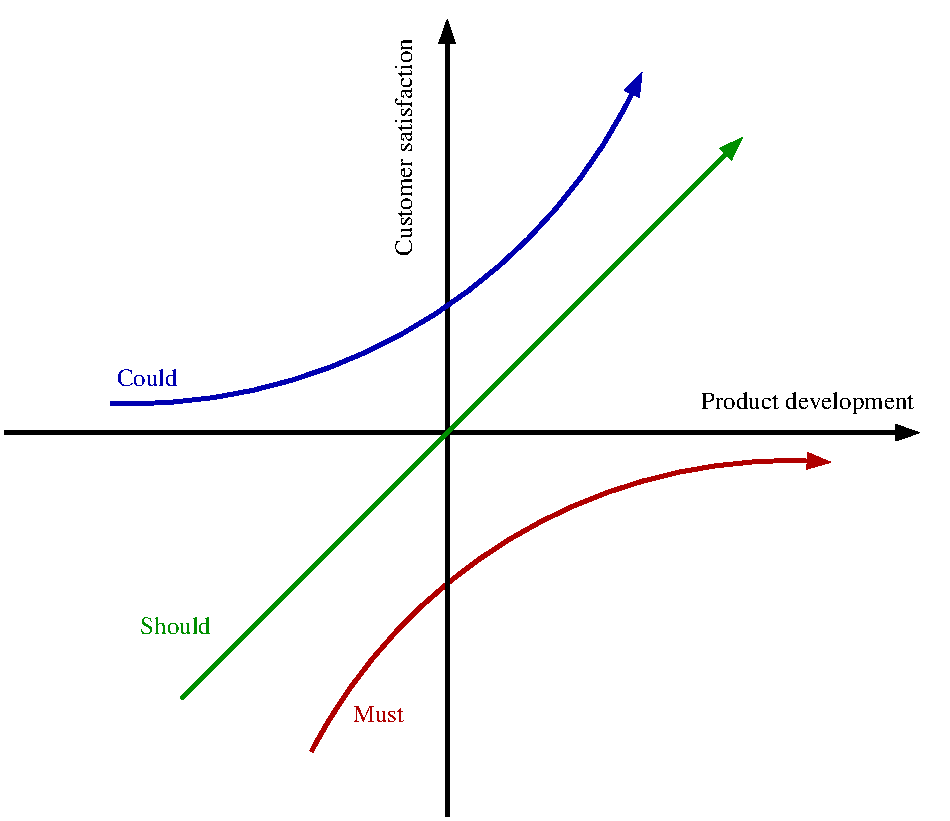
\includegraphics[width=0.65\linewidth]{kano}
  \caption{The Kano model.}
  \label{fig:kano}
\end{figure}


\emph{Validation:} In this phase, the requirements from all use case providers are collected to get the \emph{big
  picture}.  This includes a discussion among the members of the  project science review group as to the extend to which 
the
requirements can be accommodated and whether they collectively produce any potential conflicts, either internally or in
relation to the
DoW framework. Revisions and negotiations of the detailed requirements are therefore expected.  In this phase, it is 
important to ensure that Characteristic one is met.

 \emph{Evaluation and Testing:} In this phase, the focus is on the elicitation of the evaluation and testing procedures
 in the AMIDST project. This phase starts with the distribution of a new document template, where the aim is to obtain a
 high level description of the evaluation and testing methods that are necessary to measure the performance of the AMIDST
 framework. This phase is not strictly part of the RE process, but will supplement the process by providing
 detailed specifications of how to perform specific tests and evaluations. Documentation of this phase is out of the scope of 
the present document, but will
 be included in the initial version of the AMIDST handbook (Deliverable D1.3).    


\begin{figure}[htbp]
\centering
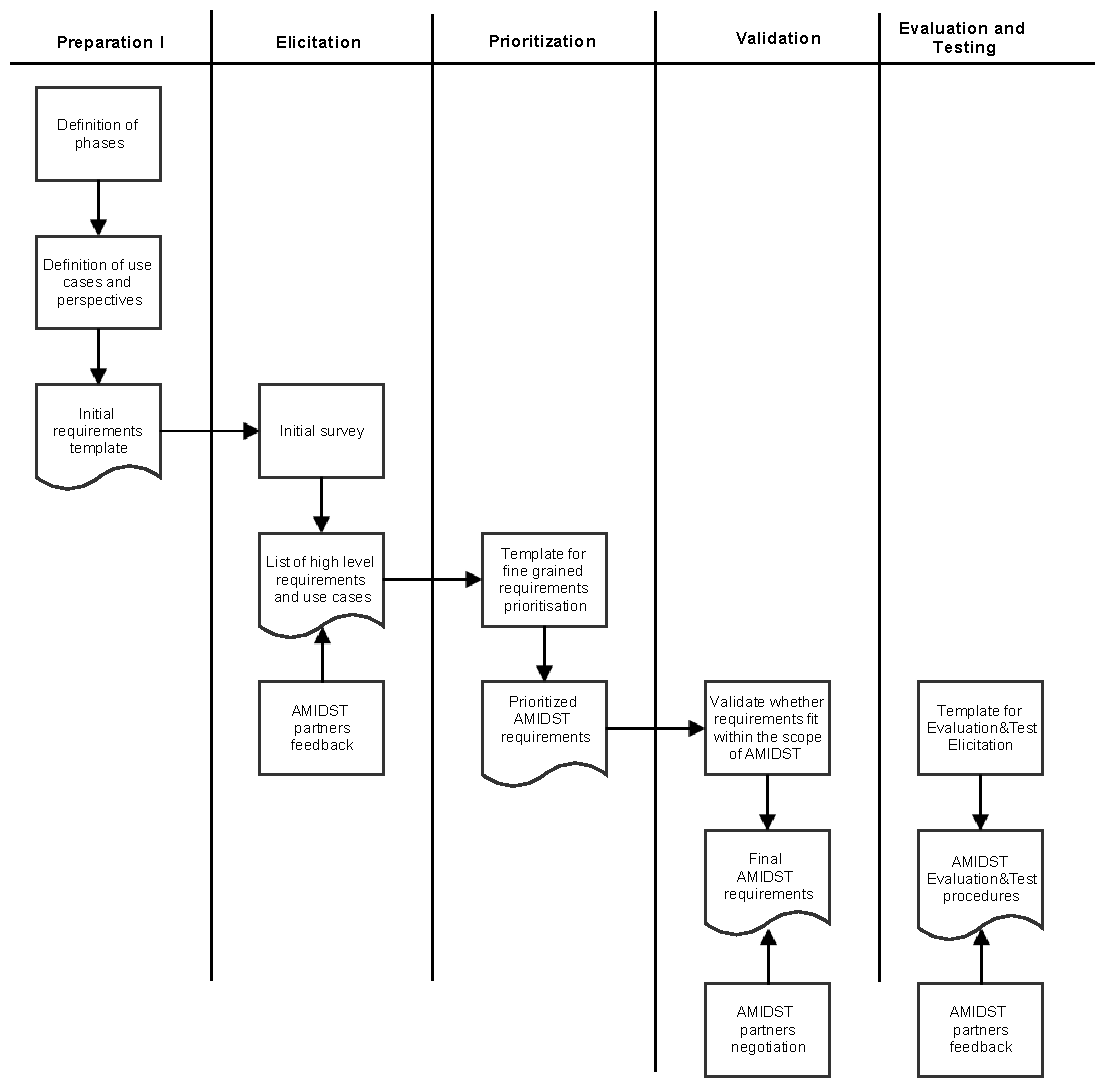
\includegraphics [keepaspectratio,width =\linewidth] {amidst_re}
\caption{Description of the five phases in the RE process in AMIDST.}
\label{REprocess1}
\end{figure}



% \subsection{Main aspects of the AMIDST's RE process}
% \label{sec:reprocess}
%
%% In this subsection, we detail the main elements that define the AMIDST RE process, which are strongly influenced by the 
%characteristics in the previous subsection.  This subsection contains a description of how the work is divided among the 
%partners and how the use case driven approach is adapted.  Moreover, a document template that is central in the AMIDST 
%RE process is described.  Requirement are discussed in terms of how they are linked with the product life cycle and 
%deliveries in the AMIDST project.  Prioritization of requirements are also briefly described, before the outline of the main 
%activities in the AMIDST RE process is given.
%


%%% Local Variables: 
%%% mode: latex
%%% TeX-master: "REproccess"
%%% End: 



\section{Realization of the requirements engineering process}
\label{sec:realization}

The RE process was organized by coupling each use case provider with an
academic partner; Verdande Technology was paired with NTNU, DAIMLER was paired with AAU and Hugin, and CajaMar was paired with
UAL. The particular partner associations were based on geographical as well as affinity
considerations. It is important to stress that the RE process does \emph{not} prescribe such a
partner association, but it does bring distinct advantages. First of all, the academic partners can better assist the use case
providers when completing the requirements template, and the ongoing internal communications and discussions (both formal
and informal) provide an opportunity for early feedback on drafts of the requirements
specification. Secondly, this division of work also provides an increased knowledge transfer between industrial and academic
partners. 

% This part of the report is written in month six when most of the process is conducted.  This section contains a few points on what experiences we have gained in the project so far:

% \begin{enumerate}
% \item Everyone involved has had a learning experience on many levels.  The industrial partners have learned about probabilistic graphical models, while the academic partners have learned about the industrial domains.  Most participants have increased their knowledge on how to conduct a requirement analysis. 
% \item There has only been one meeting where all stakeholders have met, which was the kickoff meeting in Denmark in month three.  Most communication has been done through Skype and email, but also a few face to face meetings have taken place. Most of the communications have been related to clarifications in terms of filling out the template X1.
% \item There have been adjustments of the template X1 as the process has proceeded.  Examples of this is adding fields to the requirements so they could be linked to concrete tasks in the AMIDST project or adding columns for rating the importance of a requirement.
% \end{enumerate}



% \subsubsection*{Division of work}

% For each industrial partner, a mentor among the academic partners is assigned. The mentor for Verdande Technology is NTNU, the mentor for DAIMLER is AAU; and the mentor for CajaMar is UAL. Hugin has a coordination role. On one side, this allows each of the academic partners to focus on only one industrial domain.  On the other side, the industrial partners have the academic support they need for identifying proper use cases.  This division of work is a tool to mitigate characteristic two, because it eases the knowledge transfer between the industrial and academic partners. 


As described in Section~\ref{sec:AmidstRequirementProcess} one of the design considerations for the requirements
engineering process was to base the requirements specification on a formal template that would be shared by
all three use case providers. In addition to the information that the use case providers are requested to fill-in, the
template also provides a description of the overall RE process as well as guidelines on how to
complete the template. A generic template can be found in Appendix~\ref{sec:form-fram-requ}.

  
% Because of characteristics two, we have decided to not follow a RE process that heavily relies on personal meetings and
% direct personal interviews.  Even though meetings still is an important ingredient in the process, we decided to
% distribute a document template to each of the industrial partners early in the process. 

The completion of the templates was conducted as an iterative process with a close collaboration between the use case
providers and the paired academic partners. In addition to the more formal deadlines marking transitions between 
phases in the RE process, we also introduced several short-term deadlines, where
the use case providers were given feed-back on draft versions of their completed templates. Not only did this serve as an
instrument to ensure a continuous progression in the requirements specification, where misunderstandings and problems
could be identified and mitigated at an early stage, but it also provided an early transfer of knowledge from the
industrial partners to the academic partners in the project. Part of this (otherwise tacit) knowledge were documented
for the benefit of the other partners, both current and future, in the consortium, and is expected to be included 
in the deliverables planned for Work packages 6--8. This, e.g., includes a description of the data characteristics for
the use case providers. 

% \begin{itemize}
% \item Industrial partners are pushed to contribute with use cases early, meaning that issues and misunderstandings are revealed early.  This is important to mitigate characteristic three.
% \item All ideas are documented and there is no loss of information, which is common in interviews.  This is important to meet characteristic one, three, four and five.
% \item The provided information can easily be transferred from the mentors to the other academic partners.  This is important for meeting characteristic four.
% \item  The partners can spend more time on use cases and requirements, before talking to the mentors.  To some extent, this meets characteristics three, because it is easier for the mentors to learn when the requirements are more though through.
% \item The work on the different templates can be asynchronous in time.  This eases the resources allocation for the different partners.  This is related to characteristic two.
% \end{itemize}

The specified requirements (identified by a unique label as described in Appendix~\ref{sec:form-fram-requ}) together
with their work package/task allocations and prioritizations will be summarized in
tables at the work package level. These tables allow work package leaders to get a clear overview of the specific
requirements that need to be taken into account in the different work packages. An example of a part of such a work
package requirements table can be found
in Table~\ref{tab:WP2-requirements}, which includes some of the presently collected requirements pertaining to Work package 2. 


\begin{table}[htbp]
  \centering
  \begin{tabular}{|c|c|c|c|c|}
    \hline
    Req.\ ID.\ & Relevant subphase & Must/should/could & Points & Task \\ \hline\hline
    DAI.U5.D1 & Framework devel.\ \& instan.\ & Should & 20 & 2.2  \\
    DAI.U5.D2 & Framework devel.\ \& instan.\ & Should & 20 & 2.2  \\
    DAI.U5.D3 & Framework devel.\ & Should & 15 & 2.2  \\
    DAI.U5.D4 & Framework devel.\ & Should & 15 & 2.2  \\
    DAI.U5.D4 & Framework instant.\ & Should & 20 & 2.2  \\
    DAI.U7.D1 & Framework devel.\ & Must & 35 & 2.1 \\
   \vdots & \vdots  & \vdots & \vdots & \vdots \\ \hline\hline
  \end{tabular}
  
  \caption{The work package requirements table containing the presently collected requirements for Work package 2.}
  \label{tab:WP2-requirements}
\end{table}



%%% Local Variables: 
%%% mode: latex
%%% TeX-master: "REproccess"
%%% End: 


\section{Conclusion, observations and reflections} 
% \fixme{For a
%   possible publication, we could report on our (including the use case providers') experiences with the process, but
%   since we are not yet finish with the RE process there is not that much to report \ldots }
\label{sec:conclusion}

%This document describes the requirements engineering process pursued in AMIDST as well as its application. The general process is  adapted and based
%on previously described approaches to requirements engineering, but tailored to the specific needs and characteristics of the AMIDST
%project. In particular, the idiosyncratic aspects of the AMIDST project that combined distinguishes it from other software
%projects at the RE level, include (i) a pre-defined project scope, (ii) many different
%stakeholders, and (iii) the development of a sufficiently general software framework that can be instantiated for
%use case providers representing different industries.  Central to the RE approach is the use case
%concept that forms the basis for the requirements specification. The actual specification is documented in a generic
%formal template that allows for the elicited requirements to be compared and prioritized across domains. 
%
%The division of work realized in the AMIDST project was partly successful due to the natural coupling (geographical and
%affinity based) between the industrial partners and the academic partners. This type of work division may not be
%achievable in projects with a larger number of partners or where the partners are not geographical co-located. On the
%other hand, it should also be emphasized that this division of work is \emph{not} as such prescribed by the proposed
%RE process. 
%
%The methodology that is outlined in the AMIDST project may transfer to other projects in two ways.  1) The other project share some of the same characteristics as the AMIDST project and some of the ideas are directly applicable. 2) The other project may have very different characteristics, but the very idea of identifying the key characteristics and stear RE choices based on those may be taken.  In this sence, the experiences we have had with the AMIDST project may serve as inspiration for other projects to come.

In this paper we have introduced a general methodology for the 
RE process in software development projects
with the following characteristics: relatively small group of
developers, a pre-defined project scope, stakeholders from
different industries, and the development of a general software
framework that can be instantiated according to the needs of different 
stakeholders.  The presented methodology adopts a use case-based
approach tailored to these specific characteristics of the project.
We also provide several key considerations for the RE process of this kind of project: division of the RE
approach in different phases to ease the overall implementation of
the process; structured prioritization of all the requirements to
ease the agreement between the stakeholders; and the employment of
a template based document to ease the elicitation of the
requirements and the communication between stakeholders with
different backgrounds, expectations, and locations.

In our opinion, the presented methodology is general enough to be 
applicable to a wide range of software development projects with 
similar characteristics. Concretely, we believe that the describe
RE process could be of great help to technology transfer based
projects between the academia and the industry.



\bibliographystyle{splncs}
\bibliography{re}

\end{document}  